
\FloatBarrier
\subsubsection{Система с сухим трением} % __FRIC__

\LinkRef{
  fric: ASAU-11, DSMP-2016
}

Существуют динамические системы, не обладающие хаотическим поведением,
которые, тем не менее, проявляют сходные свойства с точки зрения идентификации.
А именно, непосредственное сравнение выходов системы и модели не позволяет
сделать никаких выводов о соотношениях между параметрами модели и объекта.
Одним из примеров таких систем является динамическая система (\ref{atu:eq:dryfric_sys}),
моделирующая поведение тела заданной массы по действием внешней вынуждающей силы
и силы сухого трения
\cite{berger_friction,atu_asau11}:
%
\begin{equation}
  m \ddot{x} + f_{df}( x, \dot{x}, \ldots)  = u(t).
\label{atu:eq:dryfric_sys}
\end{equation}
%
%\noindent
где
$m$ -- масса тела,
$u(t)$ -- вынуждающая сила,
$ f_{df}( x, \dot{x}, \ldots)  $ -- сила сухого трения.

Важной особенностью при моделировании силы сухого трения является тот факт,
что это силу невозможно корректно выразить аналитически. Более того,
её алгоритмическое представления неизбежно потребует учёта всех других сил,
действующих на тело, то крайней мере, для корректного представления
силы трения покоя. Эта особенность не даёт возможности
аналитического анализа таких систем, за исключением ограниченного набора
вырожденных случаев. При этом, такое поведение существенно затрудняет идентификацию,
и, в определённых случая,х делает её принципиально невозможной.

Основным параметром, в простейшем случае определяющим силу сухого
трения, является $f_{dm}$ -- максимальная значение её модуля.
Определение этой величины и будем считать целью задачи идентификации
системы с сухим трением.

В свою очередь, существенным свойством данной системы является то, что в каждой точке \(x\)
система может находится в покое, даже если на неё действует
внешняя сила (по модулю не превышающая $f_{dm}$).
Если же рассмотреть пару или более подобных систем,
то получившаяся система имеет общие свойства с системами
хаотической динамики, а именно: малые возмущения входного сигнала
или коэффициентов модели приводят к значительным изменениям
выходного, причем реакция на возмущения может быть
не ограничена во времени.
Более того, даже если после какого-то момента времени
параметры объекта и коэффициенты модели полностью совпадут,
величина ошибки по выходнам не устремится к нулю, а останется на прежнем уровне.

На рис.~\ref{atu:f:fric_outs} представлен сравнительный пример динамики трёх
моделей, при одинаковом входном сигнале
и различных значениях $f_{dm}$.

\begin{figure}[htb!]
  \centerline{
    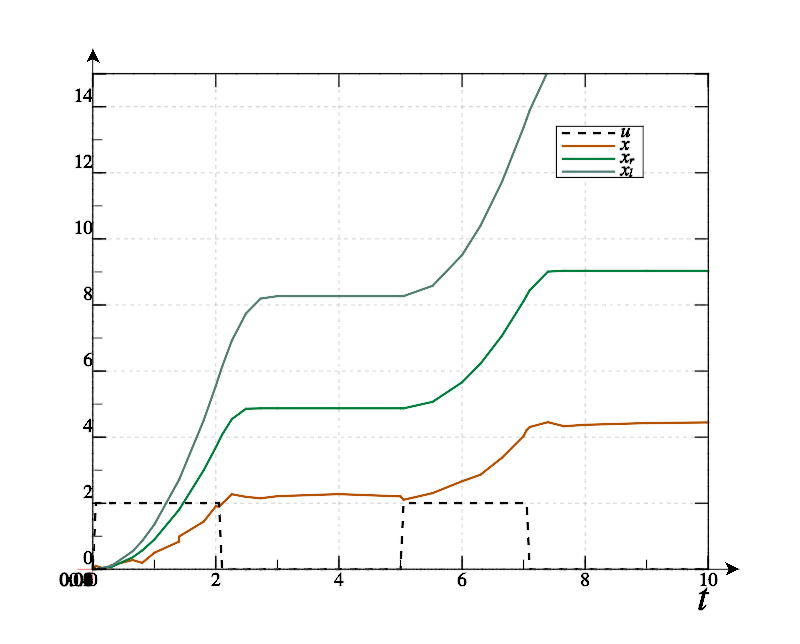
\includegraphics[width=0.5\textwidth]{p/cha/fric/fric_outs.png}
  }
  \caption{Динамика трёх моделей вида (\ref{atu:eq:dryfric_sys})}
  \label{atu:f:fric_outs}
\end{figure}

При дальнейшем моделировании, в качестве сигнала $u(t)$ использовался кусочно-линейный периодический сигнал,
в котором чередуются ``плато'' и резкие изменения. Выбор такой формы обусловлен
характерными режимами работы систем позиционирования электромеханических
устройств, для которых и характерно влияние сухого трения.

Для обеспечения возможности применения методов идентификации,
необходимо существование критерия
\( q(x(t)) \),
удовлетворяющего следующим требованиям:

\begin{itemize}

\item
чувствительность к \textit{динамике} модели и объекта;

\item
свойство астатизма, то есть
независимость
от смещения выхода объекта или модели:
\( q(x(t)+a ) \approx q( x(t) ) \);

\item
достаточная устойчивость к шумам измерения;

\item
физическая реализуемость.

\end{itemize}

Первые два требования
могут быть достигнуты путём вычисления производной --
скорости изменения выходных сигналов
\(v = \mathrm{d}\,x(t)/ \mathrm{d}\,t \),
и формирования критерия идентификации на её основе.

Однако, при этом система становится исключительно чувствительной
к шумам измерения. Даже в том случае, когда
оценка производной производится физически реализуемыми методами,
создать работоспособную систему идентификации на основе критериев
подобного вида практически невозможно.

В работе \cite{atu_asau11} был предложен метод синтеза критерия идентификации
на основе гистерезисной фильтрации выходных сигналов, с последующим
вычислением производной. Метод показал свою работоспособность, однако,
он требует достаточно точных сведений об уровне и виде шумов -- для
настройки гистерезисного фильтра. В данной работе сделаем предположение,
что уровень шумов позволяет создать фильтр, позволяющий отсеивать шумы
за (как максимум) характерное время реакции системы.
После фильтра действует реальное дифференцирующее звено.
Соответствующий вид критерия обозначим как $ q_{dx} $ (рис.~\ref{atu:f:fric_q}).



\begin{figure}[htb!]
\centerline{
  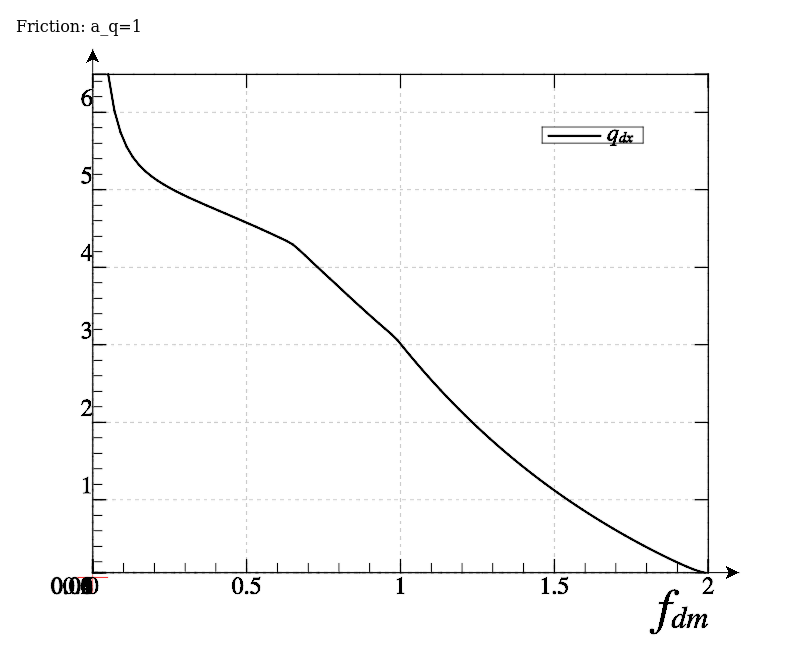
\includegraphics[width=0.50\textwidth]{p/cha/fric/fric_p-p_f_dm_q.png}
}
  \caption{Зависимость $q_{dx}(f_{dm})$ для системы (\ref{atu:eq:dryfric_sys}) }
\label{atu:f:fric_q}
\end{figure}


Динамика процессов идентификации для системы (\ref{atu:eq:dryfric_sys}) представлена на рис.~\ref{atu:f:fric_id}.
Следует отметить сильное влияние входного сигнала, В силу того, что когда системы неподвижны
на одном из ``плато'', то нет возможности различить их параметры,
какой бы критерий при этом не использовался.

\begin{figure}[htb!]
\centerline{
  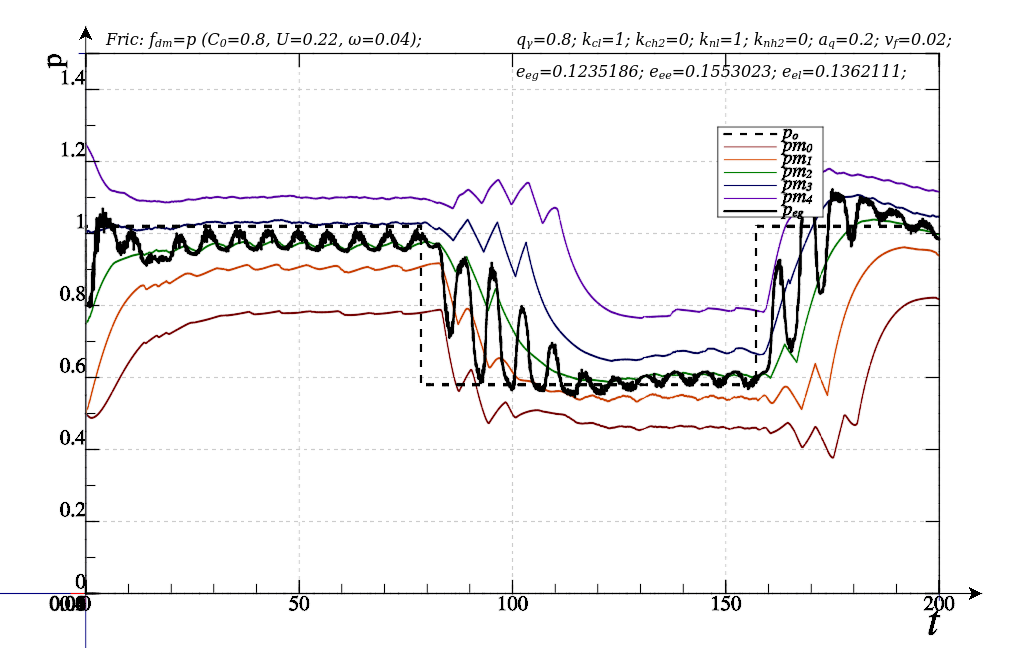
\includegraphics[width=0.49\textwidth]{p/cha/fric/fric_m5p-pl_n_sign.png}
  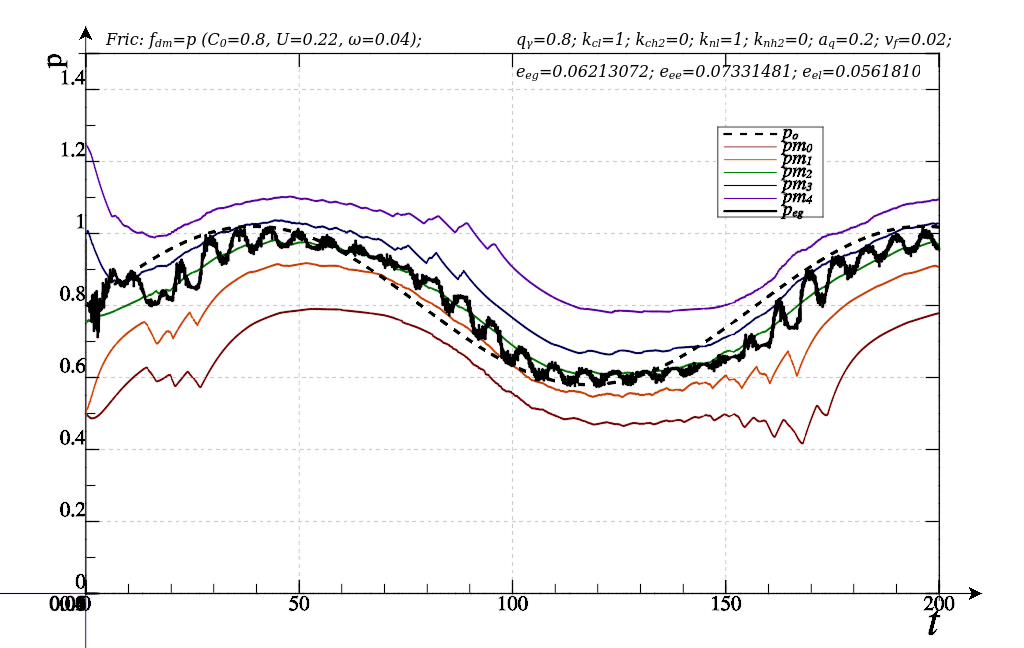
\includegraphics[width=0.49\textwidth]{p/cha/fric/fric_m5p-pl_n_sin.png}
}
\caption{Процесс идентификации параметра $c_{x_y} $ системы (\ref{atu:eq:dryfric_sys})
  при различных видах нестационарности этого параметра
}
\label{atu:f:fric_id}
\end{figure}

Зависимость среднеквадратических ошибок идентификации от величины коэффициента масштаба
$q_\gamma$ (рис.~\ref{atu:f:fric_e_qgamma})
достаточно сильно отличатся от аналогичной, например, для системы ``Sprott A''. На ней явно выражены
экстремумы, дающие возможность тонкой настройки системы идентификации. Следовательно,
для данной динамической системы робастные свойства системы идентификации проявляются слабо,
и может потребовался дополнительная адаптация.

\begin{figure}[htb!]
\centerline{
  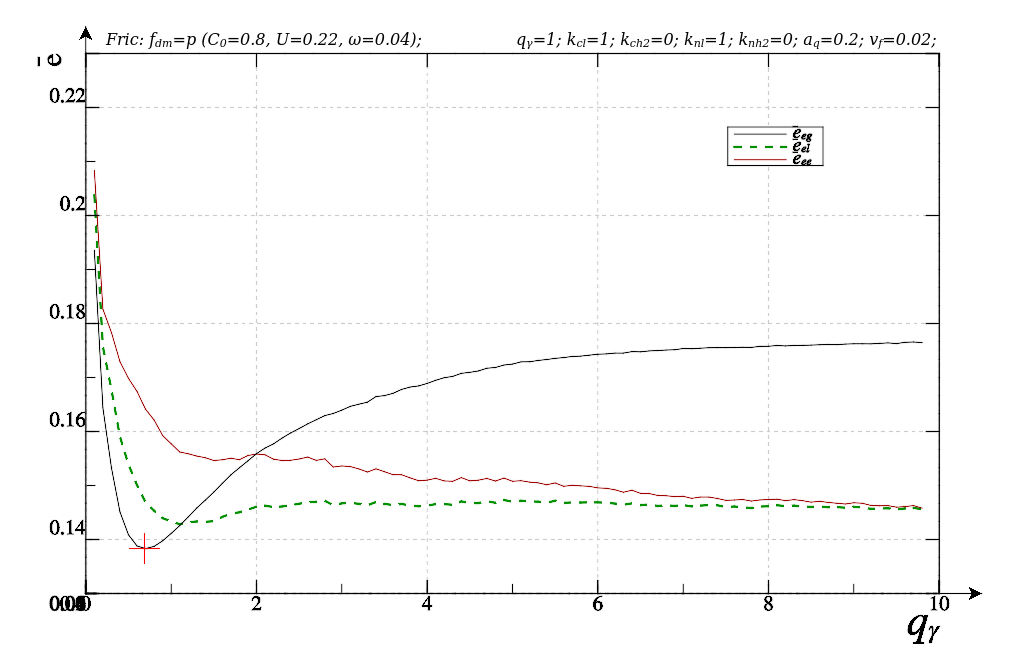
\includegraphics[width=0.49\textwidth]{p/cha/fric/fric_m5p-p_qg_e_sign.png}
  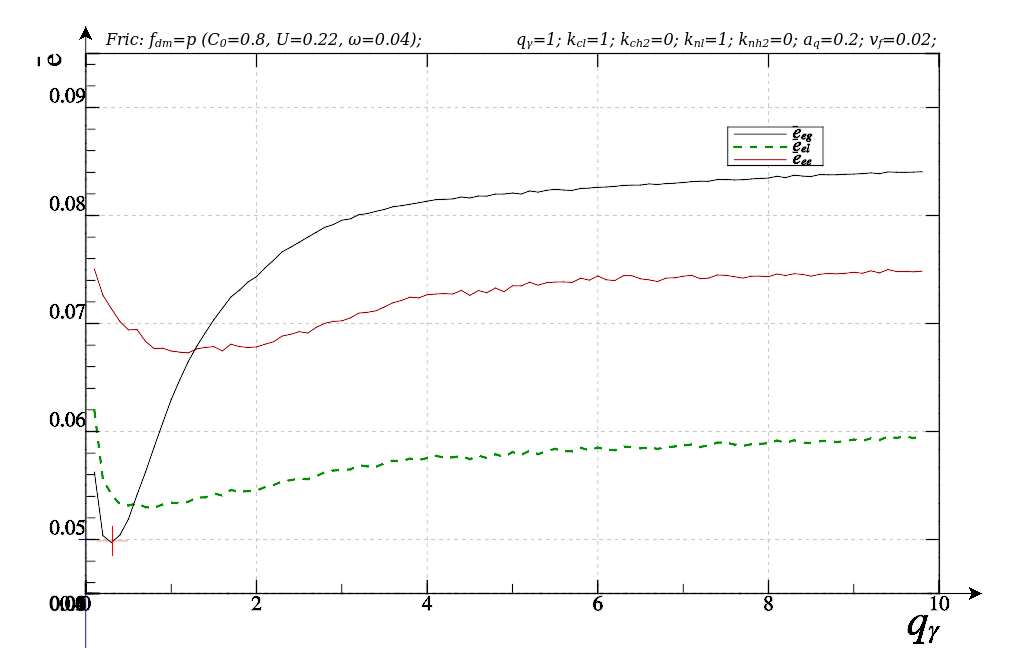
\includegraphics[width=0.49\textwidth]{p/cha/fric/fric_m5p-p_qg_e_sin.png}
}
  \caption{Зависимости  $\overline{e}(q_\gamma)$ для системы (\ref{atu:eq:dryfric_sys})
  при различных видах нестационарности этого параметра
}
\label{atu:f:fric_e_qgamma}
\end{figure}


Зависимости $\overline{e_*}(a_q)$ (рис.~\ref{atu:f:fric_e_a_q})
 позволяют корректно определить время усреденения.

\begin{figure}[htb!]
\centerline{
  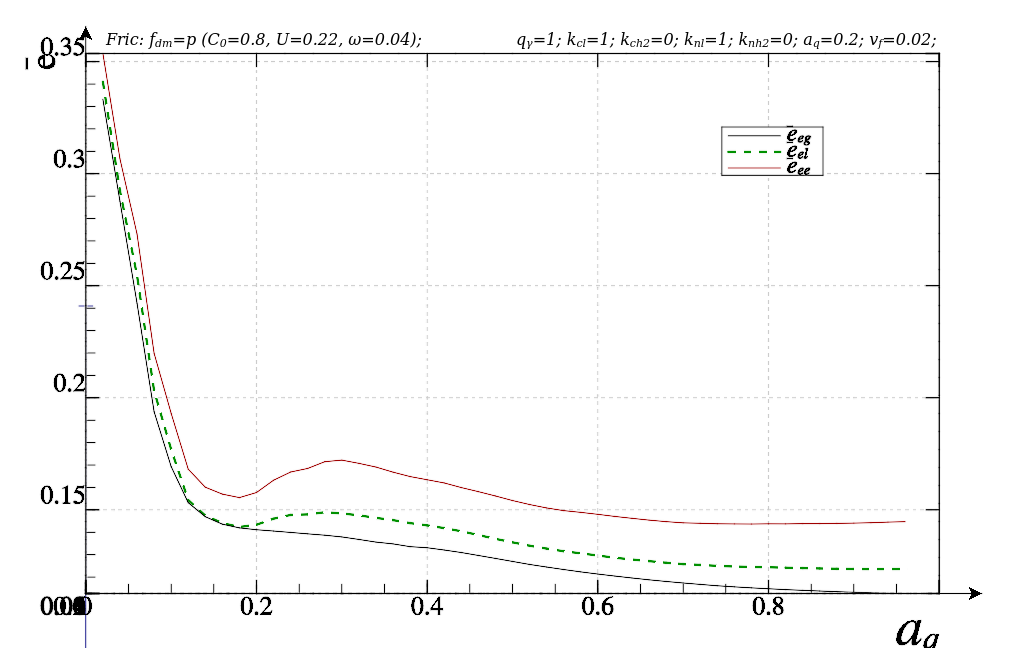
\includegraphics[width=0.49\textwidth]{p/cha/fric/fric_m5p-p_a_q_e_sign.png}
  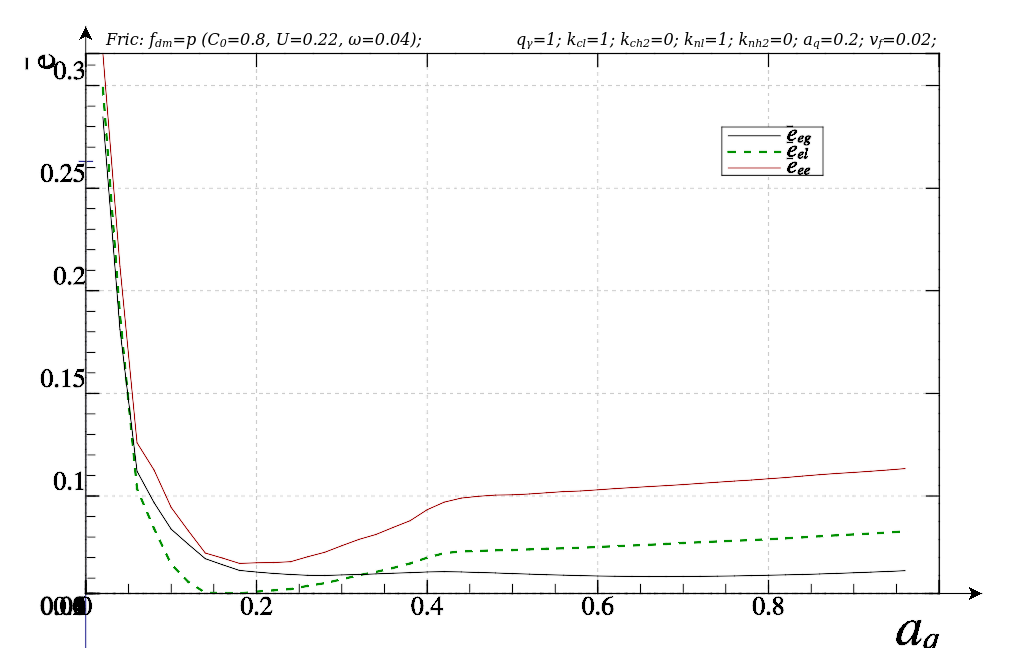
\includegraphics[width=0.49\textwidth]{p/cha/fric/fric_m5p-p_a_q_e_sin.png}
}
  \caption{Зависимости  $\overline{e}(a_q)$ для системы (\ref{atu:eq:dryfric_sys})
  при различных видах нестационарности этого параметра
}
\label{atu:f:fric_e_a_q}
\end{figure}

Для данной системы энергетические критерии, аналогичные применённым в предыдущих случаях,
оказались неприменимы. Критерий, хоть и основанный на измерении производной (после фильтрации),
оказался работоспособным. В первую очередь это связано с тем, что в основе были положены
физические принципы, которые для системы с сухим трением, вполне очевидны.

